\documentclass[12pt]{article}
\usepackage[margin=1in,letterpaper]{geometry}
\usepackage[utf8]{inputenc}
\usepackage[T1]{fontenc}
\usepackage{graphicx}
\usepackage{amssymb}
\usepackage{amsmath}
\usepackage{palatino}
\usepackage{mathpazo}
\usepackage{color}
\usepackage{hyperref}
\usepackage{multirow}
\usepackage{braket}
\usepackage{relsize}
\usepackage{color, colortbl}
\usepackage{booktabs}
\usepackage[dvipsnames]{xcolor}
\definecolor{darkblue}{RGB}{46,48,147}
\hypersetup{colorlinks=true,
            linkcolor=darkblue,
            urlcolor=darkblue,
            citecolor=darkblue}
\definecolor{Gray}{gray}{0.9}
\definecolor{LightCyan}{rgb}{0.88,1,1}
\definecolor{LightRed}{rgb}{1,0.92,0.92}
\newcommand{\solColor}{blue}
\newcommand{\sol}{\color{\solColor}}
\newcommand*\publistbasestyle{phys}
\usepackage[style=publist,
biblabel=brackets,
sorting=dt,
plauthorhandling=highlight,
nameorder=given-family,
]{biblatex}
\DeclareSourcemap{
 \maps[datatype=bibtex,overwrite=true]{
  \map{
    \step[fieldsource=Collaboration, final=true]
    \step[fieldset=usera, origfieldval, final=true]
  }
 }
}
\renewbibmacro*{author}{
  \iffieldundef{usera}{
    \printnames{author}
  }{
    \printfield{usera} Collaboration
  }
}
\addbibresource{syllabus.bib}

\begin{document}

\begin{center}
	\textbf{University of California San Diego\\
		Department of Physics\\
		Physics 139/239, Fall 2025\\
		Machine Learning in Physics (4 units)}
\end{center}

\begin{figure}[h!]
	\centering
	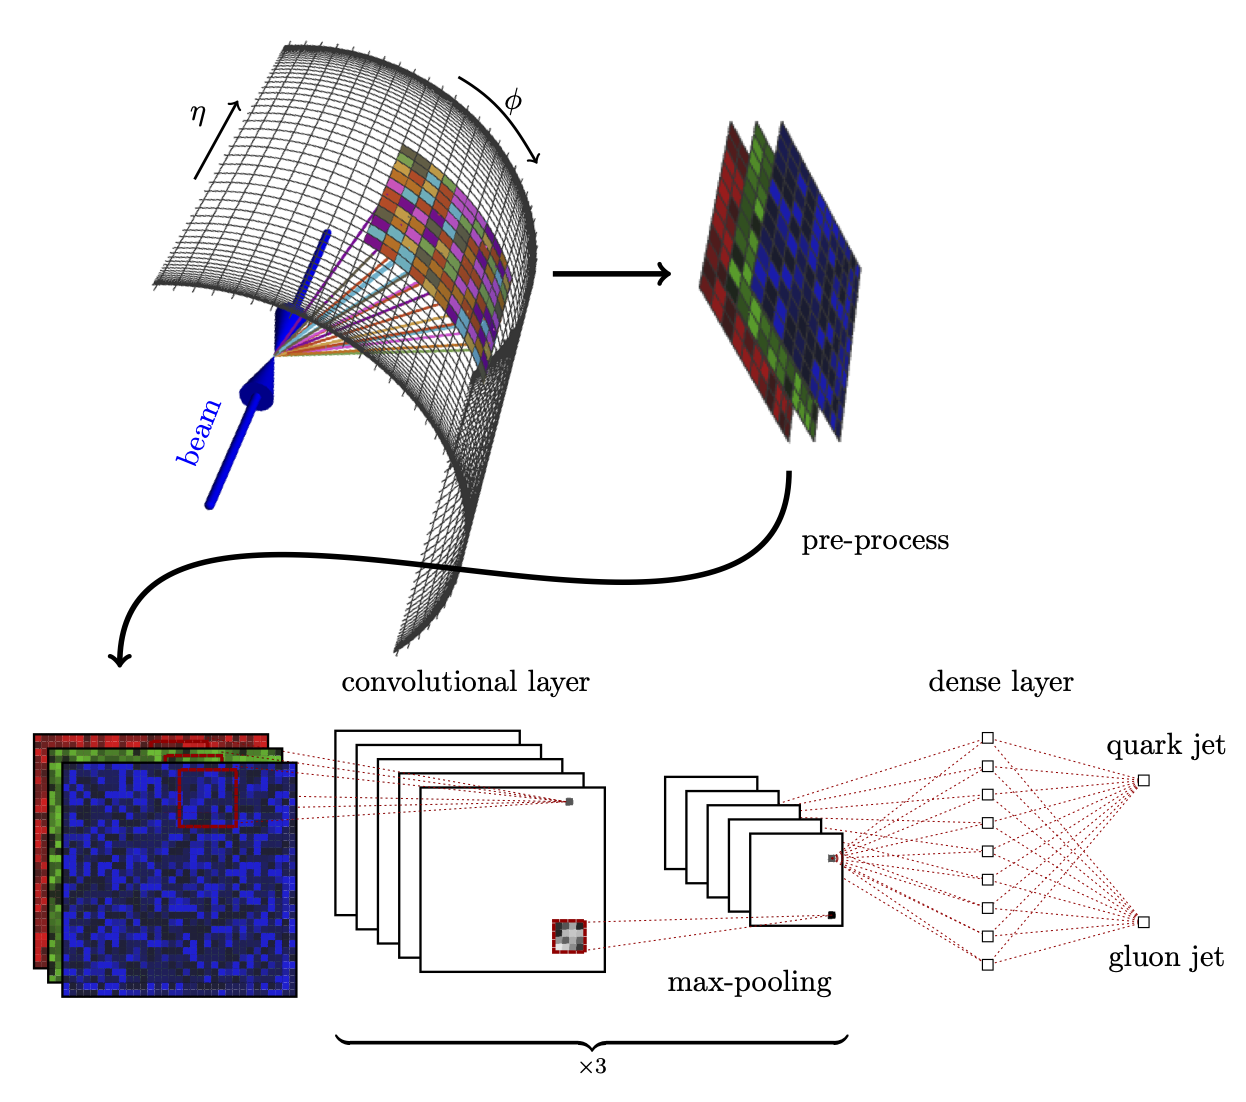
\includegraphics[width=0.7\textwidth]{quark_gluon.pdf}
\end{figure}

\noindent\textbf{Instructor}: Javier Duarte, \href{mailto:jduarte@ucsd.edu}{jduarte@ucsd.edu}, OH by appt. MYR-A 5516 \\
\noindent \textbf{Teaching assistant}: Daniel Primosch, \href{mailto:dprimosc@ucsd.edu}{dprimosc@ucsd.edu}, OH Tu 4--5:00pm MYR-A 5516

\noindent\textbf{Course webpage, Zoom link to lectures}:\\
\hspace*{1cm}Canvas: \href{https://canvas.ucsd.edu/courses/56257}{https://canvas.ucsd.edu/courses/56257}\\
\hspace*{1cm}Webpage: \href{https://jduarte.physics.ucsd.edu/phys139\_239}{https://jduarte.physics.ucsd.edu/phys139\_239}\\
\hspace*{1cm}All assignments will be due through Gradescope (accessed through Canvas).

\begin{center}
	\rule{\textwidth}{0.5pt}
\end{center}

\noindent\textbf{Course information}: This course is an upper-division undergraduate course and introductory graduate course on machine learning in physics.
No previous machine learning knowledge is necessary.
However, some basic knowledge of calculus, linear algebra, statistics, and Python programming may be expected/useful.

The course structure will consist of weekly lectures on conceptual topics, e.g. statistics, linear algebra, scientific data set exploration, feature engineering, (stochastic) gradient descent, neural networks, and unsupervised learning.
Students will learn key concepts in data science and machine learning, including selecting and preprocessing data, designing machine learning models, evaluating model performance, and relating model inputs and outputs to the underlying physics concepts.
We will apply these methods to the domains of collider physics, neutrino physics, astronomy, and potentially others.
There will be 4 homework assignments.
There will also be a final project in which students will work in groups to reproduce the results of an ML in physics research article.
A midterm assignment to propose the project will also be required.

\begin{center}
	\rule{\textwidth}{0.5pt}
\end{center}

\noindent\textbf{Schedule}:
\begin{center}
	\begin{tabular}{|l|c|l|m{60mm}|}
		\hline
		Lecture    & MWF           & 12--12:50p   & RWAC	0121, Zoom \href{https://ucsd.zoom.us/j/96709322126}{96709322126}  \\\hline
		Final exam & Th 12/11/2025 & 11:30a-2:29p & RWAC 0121, Zoom \href{https://ucsd.zoom.us/j/96709322126}{96709322126} \\\hline
	\end{tabular}
\end{center}

\noindent\textbf{First lecture}: F 9/26/2025

\noindent{\textbf{Pre-course survey}}: Please fill out this \href{https://canvas.ucsd.edu/courses/69038/quizzes/227768}{pre-course survey} and attest that you have done it on Canvas by 9/26/2025.

\begin{center}
	\rule{\textwidth}{0.5pt}
\end{center}

\noindent\textbf{Textbook}: There is no required textbook for this course.
At the end of the syllabus, we list a bibliography of (mostly free) textbooks and online resources we will draw from.

\begin{center}
	\rule{\textwidth}{0.5pt}
\end{center}

\noindent\textbf{Student learning outcomes}: Upon successful completion of Physics 139/239, students will be able to:
\begin{itemize}
	\itemsep-0.3em
	\item Find, explore, select, and preprocess scientific data
	\item Choose and design machine learning models
	\item Evaluate model performance and compare to standard benchmarks
	\item Debug machine learning workflows
	\item Relate model inputs and outputs to underlying physics concepts
	\item Collaborate with peers to tackle complex, realistic problems
	\item Present findings
\end{itemize}

\begin{center}
	\rule{\textwidth}{0.5pt}
\end{center}

\noindent\textbf{Grading policy}: Your final course grade will be determined according to the following:
\begin{itemize}
	\itemsep-0.3em
	\item 50\% Homework.
	\item 10\% Participation and attendance.
	\item 20\% Midterm: Written proposal for group project.
	\item 20\% Final: Written group project summary, presentation, self/peer evaluations, and code.
\end{itemize}

\begin{center}
	\rule{\textwidth}{0.5pt}
\end{center}

\noindent\textbf{Drop policy}: The lowest homework score is dropped automatically.
This drop policy is designed to account for any illnesses, family, medical, mental, or other emergencies.

If you have an extended emergency (e.g., a long hospital stay) that hinders your ability to turn complete assignments beyond the emergency policy allowance, contact the professor directly as soon as the situation arises.

\begin{center}
	\rule{\textwidth}{0.5pt}
\end{center}

\noindent\textbf{Discussion board}: We will use Slack: \href{https://join.slack.com/t/ucsdphys139/shared\_invite/zt-110gwd4lx-pZBsItfcxhbOD5BV6afVDA}{ucsdphys139.slack.com}

\begin{center}
	\rule{\textwidth}{0.5pt}
\end{center}

\noindent\textbf{Homework}: Each homework will consist of a set of conceptual and programming problems.
The assignments will be submitted as Jupyter notebooks or GitHub repositories.

There will be a first deadline (on Fridays at 8:00pm) to submit the homework, which will be graded based on effort and completeness.

There will be a second deadline (on Wednesdays at 8:00pm) to submit corrections for the homework, which will be graded based on effort and correctness.
You are required to submit corrections for all assignments even if you believe everything is correct.
In that case, for each problem, you should indicate that you've checked the solution and your solution is equivalent.

\begin{center}
	\rule{\textwidth}{0.5pt}
\end{center}

\noindent\textbf{Midterm and final project}:
For the final project, students will work in groups of $\sim$4 to reproduce or extend the results of an ML in physics research article.
Some candidate articles are listed at the end of the syllabus.
The final project deliverables are: (1) a 4-page paper on the project, (2) code provided as a public GitHub repository, (3) a 10-minute presentation by all members of the group during finals week, and (4) self and peer evaluations for group contributions.
Students will also be required to submit a 1-page written proposal for the project in Week 7.
This is to ensure the project is feasible and to receive feedback from the instructors.

\begin{center}
	\rule{\textwidth}{0.5pt}
\end{center}

\noindent\textbf{Attendance (lectures)}: In-person lecture attendance is strongly recommended and worth 10\% of your grade.
To record your attendance, write your name on the whiteboard or chalkboard at the beginning of lecture.
The full 10\% will be awarded for attending 80\% of the lectures.
The lecture hours will be split into conceptual and hands-on portions, with interactive problem-solving and pair programming throughout.
Please, bring a laptop that you can program with to lecture.
If you do not have one, please contact the instructor, and we will help you.
These sessions will be recorded.

\emph{Exit tickets}: At the end of each class, you will be invited to fill out an \href{https://forms.gle/4DmG5SjBUEM5pe6U8}{exit ticket}.


\begin{center}
	\rule{\textwidth}{0.5pt}
\end{center}

\noindent\textbf{Academic integrity (including AI tools, e.g. ChatGPT)}: Please read the College Policies section of the \href{http://senate.ucsd.edu/Operating-Procedures/Senate-Manual/Appendices/2}{UCSD's Policy on Integrity of Scholarship}.
These rules will be enforced.
Cheating includes, but is not limited to: submitting another person's work as your own, copying from any person/source, and using any unauthorized materials or aids during exams.

We understand that many of you may utilize AI tools such as ChatGPT to assist with your coursework.
While these tools can be valuable resources for learning and exploring concepts, it is important to use them responsibly.
Copying and pasting AI-generated answers without making an effort to understand the material not only undermines your learning but also violates the principles of academic integrity.
Although we can often identify the use of such tools, we recognize that some instances may go undetected.
Relying solely on these tools without comprehension will hinder your long-term academic and professional development.
We encourage you to use AI assistance to enhance your understanding and support your problem-solving processes, but ensure that all submitted work reflects your own effort and comprehension.

Copying from an online solution, a peer's solution, a Chegg solution, or shared work (on Slack, for example) is considered cheating.
Collaboration is encouraged, but by the time you start writing your own solution to turn in, you should not be looking at any other source.
You should know the rough outline of the solution well enough that you do not need to reference something line-by-line.
Plagiarizing a solution but changing variable names is considered cheating.
Soliciting help online via Chegg, Quora, etc. is considered cheating.
If suspected, you might be asked to rework similar problems in a Zoom one-on-one meeting with the instructor and/or TA.

Any questions on what constitutes an academic integrity violation should be addressed to the instructor; any violation of academic integrity will result in immediate reporting to the UCSD Office of Academic Integrity, and can result in an automatic ``F'' for the course at the discretion of the instructor.

\begin{center}
	\rule{\textwidth}{0.5pt}
\end{center}

\noindent\textbf{Counseling and Psychological Services (CAPS):} The mission of CAPS is to promote the personal, social, and emotional growth of students.
Many services are available to UCSD students including individual, couples, and family counseling, groups, workshops, and forums, consultations and outreach, psychiatry, and peer education.
To make an appointment, call (858) 534-755.
For more information, visit \href{https://wellness.ucsd.edu/caps/}{https://wellness.ucsd.edu/caps/}.

\begin{center}
	\rule{\textwidth}{0.5pt}
\end{center}

\noindent\textbf{\emph{Schedule}} (Subject to change):\\

\noindent\textbf{Week 0}

\emph{Friday 9/26}: \underline{Lecture 01}: Course overview, introduction to ML, linear regression; Homework 1 released

\noindent\textbf{Week 1}

\emph{Monday 9/29}: \underline{Lecture 02}: Introduction to ML, linear regression (cont.)

\emph{Wednesday 10/1}: \underline{Lecture 03}: Over/underfitting, bias-variance tradeoff, cross validation

\emph{Friday 10/3}: \underline{Lecture 04}: Perceptron learning algorithm, (stochastic) gradient descent; \underline{Hands-on}: Python/Jupyter, NumPy, Git, debugging

\noindent\textbf{Week 2}

\emph{Monday 10/6}: \underline{Lecture 05}: Support vector machine

\emph{Wednesday 10/8}: \underline{Lecture 06}: Regularization, logistic regression

\emph{Friday 10/10}: Homework 1 due; \underline{Lecture 07}: (Boosted) decision trees

\noindent\textbf{Week 3}

\emph{Monday 10/13}: \underline{Lecture 08}: (Boosted) decision trees (cont.); \underline{Hands-on}: Scikit-learn, XGBoost, classifying Higgs boson events

\emph{Wednesday 10/15}: Homework 1 (corrections) due; Homework 2 released; \underline{Lecture 09}: (Deep) neural networks, backpropagation

\emph{Friday 10/17}: \underline{Lecture 10}: Classification metrics, confusion matrix, ROC curve, AUC

\noindent\textbf{Week 4}

\emph{Monday 10/20}: \underline{Lecture 11}: (Deep) neural networks (cont.), training issue, data standardization; \underline{Hands-on}: Keras, classifying jets with high-level features

\emph{Wednesday 10/22}: \underline{Lecture 12}: Optimizers: (Nesterov) momentum, RMSProp, Adam, skip connections, regularization: dropout, early stopping

\emph{Friday 10/24}: Homework 2 due; \underline{Lecture 13}: Types of data, inductive bias, image-like data, convolutional neural networks

\noindent\textbf{Week 5}

\emph{Monday 10/27}: \underline{Lecture 14}: Convolutional neural networks (cont.)

\emph{Wednesday 10/29}: Homework 2 (corrections) due; Homework 3 released; \underline{Lecture 15}: Spherical convolutional neural networks

\emph{Friday 10/31}: \underline{Hands-on}: Keras, classifying astronomical data (images)

\noindent\textbf{Week 6}

\emph{Monday 11/3}: \underline{Lecture 16}: Time-series data, recurrent neural networks

\emph{Wednesday 11/5}: \underline{Lecture 17}: Recurrent neural networks (cont.)

\emph{Friday 11/7}: Homework 3 due; \underline{Hands-on}: Identifying radio signals (time series)

\noindent\textbf{Week 7}

\emph{Monday 11/10}: \underline{Lecture 18}: Point cloud and graph-like data, relational inductive bias, permutation invariance/equivariance, graph neural networks and transformers

\emph{Wednesday 11/12}: Homework 3 (corrections) due; \underline{Lecture 19}: Graph neural networks and transformers (cont.)

\emph{Friday 11/14}: Project proposal due; \underline{Hands-on}: Graph neural networks and transformers, $N$-body simulations, springs

\noindent\textbf{Week 8}

\emph{Monday 11/17}: \underline{Lecture 21}: Unsupervised learning, clustering

\emph{Wednesday 11/19}: \underline{Lecture 22}: Autoencoders, variational autoencoders

\emph{Friday 11/21}: Homework 4 due; \underline{Lecture 23}: Generative modeling; \underline{Hands-on}: Finding anomalies in LHC/LIGO data

\noindent\textbf{Week 9}

\emph{Monday 11/24}: \underline{Lecture 24}: Model compression, pruning

\emph{Wednesday 11/26}: Homework 4 (corrections) due; \underline{Lecture 25}: Quantization, knowledge distillation; \underline{Hands-on}: TensorFlow Model Optimization, QKeras

\noindent\textbf{Week 10}

\emph{Monday 12/1}: \underline{Lecture 26}: Large language models and foundation models

\emph{Wednesday 12/3}: \underline{Lecture 27}: Large language models and foundation models (cont.); \underline{Hands-on}: Fine-tuning LLMs

\emph{Friday 12/5}: \underline{Guest lecture}: TBD

\noindent\textbf{Finals Week}

\emph{Thursday 12/11}: Final presentations and projects due

\begin{center}
	\rule{\textwidth}{0.5pt}
\end{center}

\noindent\textbf{\emph{Bibliography}}:\\

\textbf{Textbooks:}

\newrefsection
\nocite{Mehta:2019,Abu-Mostafa:2012,Erdman:2021,Zeljko:2014,Calafiura:2022,Chollet:2021,Goodfellow-et-al-2016}
\printbibliography[heading=none]

\textbf{Videos:}

\newrefsection
\nocite{3blue1brown_neuralnetwork,3blue1brown_gradientdescent}
\printbibliography[heading=none]

\textbf{Reviews:}

\newrefsection
\nocite{Carleo:2019ptp,hepmllivingreview,ParticleDataGroup:2024cfk}
\printbibliography[heading=none]

\textbf{Candidate articles for final project:}

\newrefsection
\nocite{deOliveira:2015xxd,Aurisano:2016jvx,Komiske:2016rsd,Khan:2018opv,Zhou:2019,Moreno:2019neq,Ormiston:2020ele,Moreno:2021fvp,Erdmann:2019nie,Guest:2016iqz,Majorana:2023kmv,Fry:2024lcg,Miao:2024oqy,Li:2024htp,LSSTDarkEnergyScience:2019cvx}
\printbibliography[heading=none]

\textbf{Public datasets:}

\newrefsection
\nocite{kasieczka_gregor_2019_2603256,hbb_dataset,galaxy-zoo-the-galaxy-challenge,g2net-gravitational-wave-detection,trackml-particle-identification,majorana_collaboration_2023_8257027,jetclass,jetclass2,plasticc-kaggle}
\printbibliography[heading=none]

\end{document}
